\documentclass[UTF8,a4paper,11 pt]{ctexart}%字符标准,纸张,字体大小,文档类型,自行打印11pt,单位打印12pt
\usepackage{mathtools,amssymb,array,amsthm,amsmath}%数学宏包
\usepackage{geometry,ulem,graphicx,longtable,caption2,cite,fancyhdr,multicol,color}%通用宏包
\geometry{a4paper,left=1.5cm, right=1.5cm, top=2.6cm, bottom=3cm}%页面布局
\usepackage{siunitx,xfp,empheq,unicode-math,xchoices}
\sisetup{
	separate-uncertainty = true,
	inter-unit-product = \ensuremath{{}\cdot{}}
}%单位及预设
\usepackage{chemfig,mhchem}%化学宏包
\newcommand\dif{\mathop{}\!\mathrm{d}}%定义微分算子
\newcommand\eu{\mathrm{e}}%定义自然常数
%\renewcommand\bar{\overline}
%\renewcommand\vec{\overrightarrow}
\everymath{\displaystyle}%行间公式
\usepackage{xeCJK,wrapfig,text-figure}
\usepackage[hidelinks]{hyperref}
\xeCJKsetup{
	CJKecglue={\:}
}
\AtBeginDocument{
	\let\mathbb\relax
	\DeclareMathAlphabet{\mathbb}{U}{msb}{m}{n}
}
\usetikzlibrary{decorations.pathmorphing,patterns}
\usetikzlibrary {patterns.meta}
\setlength{\lineskip}{8pt}
\setlength{\lineskiplimit}{8pt}
\begin{document}
	\setlength{\lineskip}{8pt}
	\setlength{\lineskiplimit}{8pt}
	\pagestyle{fancy}
	\fancyhead[L]{\leftmark}%左页眉,section
	\fancyhead[R]{Written By Feizao From Class 5 With \LaTeX}%右页眉,subsection
	%\fancyfoot[L]{Written By Feizao With \LaTeX} %左页脚
	%\fancyfoot[R]{\thepage} %右页脚
	\fancyhead[C]{} %中页脚
	\fancyfoot[C]{}
	\title{\textbf{每周习题}} %标题
	\author{Written By Feizao With \LaTeX}
	\date{}
	\maketitle
	\tableofcontents %目录
	\section{第一周}%无
	\clearpage\section{第二周の遗物}
	\subsection{D1-T1}\noindent
	如图所示,质量$ m_c=2m_b $的物块$ c $静止在倾角$ \alpha=30^\circ $的等腰斜面上的$ E $点,质量为$ m_a $的物块$ a $和质量为$ m_b $的物块$ b $通过一根不可伸长的匀质细绳相连,细绳绕过斜面顶端的小滑轮并处于松弛状态,按住物块$ a $使其静止在$ D $点,让物块$ b $从斜面顶端$ C $静止下滑,刚下滑碰到$ E $点时释放物块$ a $,细绳刚好伸直并瞬间张紧绷断,之后物块$ b $与$ c $立即发生完全弹性碰撞,碰后物块$ a,b $都经过$ t=\SI{1}{s} $同时到达斜面底端. 已知$ A,D $两点和$ C,E $两点的距离$ l_1=\SI{0.9}{m} $,$ E,B $两点的距离$ l_2=\SI{0.4}{m} $. 斜面上除$ EB $段以外其余都是光滑的,物块$ b,c $与$ EB $段的动摩擦因数$ \mu=\dfrac{\sqrt{3}}{3} $,空气阻力不计,滑轮处摩擦不计,细绳张紧时与斜面平行,取重力加速度$ g=\SI{10}{m/s^2} $. 求:
	\begin{figure}[htp]
		\centering
		\begin{tikzpicture}[scale=1.5]
			\draw (0,0)to(-30:6)node[right]{$ B $};
			\draw (0,0)to(210:6)node[left]{$ A $};
			\draw (-{sqrt(27)},-3) to ({sqrt(27)},-3);
			\draw ({54/13*cos(30)},-{54/13*sin(30)})node[below]{$ E $}to({54/13*cos(30)+6/13*sin(30)},{6/13*cos(30)-54/13*sin(30)});
			\draw ({60/13*cos(30)},{-60/13*sin(30)})to({60/13*cos(30)+6/13*sin(30)},{6/13*cos(30)-60/13*sin(30)});
			\draw ({54/13*cos(30)+6/13*sin(30)},{6/13*cos(30)-54/13*sin(30)})to({60/13*cos(30)+6/13*sin(30)},{6/13*cos(30)-60/13*sin(30)});
			\node at ({27/13*cos(30)+30/13*cos(30)+3/13*sin(30)},{3/13*cos(30)-30/13*sin(30)-27/13*sin(30)}) {$ c $};
			\draw ({6/13*cos(30)},-{6/13*sin(30)})to({6/13*cos(30)+6/13*sin(30)},{6/13*cos(30)-6/13*sin(30)});
			\draw ({12/13*cos(30)},{-12/13*sin(30)})to({12/13*cos(30)+6/13*sin(30)},{6/13*cos(30)-12/13*sin(30)});
			\draw ({6/13*cos(30)+6/13*sin(30)},{6/13*cos(30)-6/13*sin(30)})to({12/13*cos(30)+6/13*sin(30)},{6/13*cos(30)-12/13*sin(30)});
			\node at ({3/13*cos(30)+6/13*cos(30)+3/13*sin(30)},{3/13*cos(30)-6/13*sin(30)-3/13*sin(30)}){$ b $};
			\draw ({-4*6/13*cos(30)},{-4*6/13*sin(30)})node[below]{$ D $}--({-4*6/13*cos(30)-6/13*sin(30)},{-4*6/13*sin(30)+6/13*sin(60)})--({-5*6/13*cos(30)-6/13*sin(30)},{-5*6/13*sin(30)+6/13*sin(60)})--({-5*6/13*cos(30)},{-5*6/13*sin(30)});
			\node at ({-2*6/13*cos(30)-3/13*sin(30)-5*6/26*cos(30)},{-2*6/13*sin(30)+3/13*sin(60)-5*3/13*sin(30)}){$ a $};
			\draw (0,0) to(90:2/13);
			\draw (0,2/13) circle (3/26);
			\node at (-1/3,6/13) {$ C $};
			\draw ({3/26*sin(30)},{3/26*cos(30)+2/13}) to({3/26*sin(30)+1.75/26+6/13*sin(60)},{3/26*cos(30)+2/13-1.75/26*tan(30)-6/13*sin(60)*tan(30)});
			\draw (-3/26,2/13) .. controls ({-24/13*sin(30)},{-24/13*sin(60)}) .. ({-4*6/13*cos(30)-3/13*sin(30)},{-4*6/13*sin(30)+3/13*sin(60)});
			\draw (-4.5,-3) arc (0:30:{6*sin(60)-4.5});
			\draw (4.5,-3) arc (180:150:{6*sin(60)-4.5});
			\node at ({-6*sin(60)+0.9*cos(15)},{0.9*sin(15)-3}) {$ \alpha $};
			\node at ({6*sin(60)-0.9*cos(15)},{0.9*sin(15)-3}) {$ \alpha $};
		\end{tikzpicture}
	\end{figure}
	\\(1)物块$ b $由$ C $点下滑至$ E $点所用时间;\\
	(2)物块$ a $能到达离$ A $点的最大高度;\\
	(3)物块$ a,b $的质量比$ \dfrac{m_a}{m_b} $.
	\\\quad\\\quad\\\quad\\\quad\\\quad
	\subsection{D2-T2}\noindent
	已知非负实数$ x,y $满足$ x^2+4y^2+4xy+4x^2y^2=32 $,则$ \sqrt{7}(x+2y)+2xy $的最大值为\underline{\qquad\qquad}.
	\clearpage\subsection{D3}
	\subsubsection{T3}
	\noindent 如图所示,用跨过光滑滑轮的轻质细绳将小船沿直线拖向岸边,已知拖动细绳的电动机功率恒为$ P $,电动机卷绕绳子的轮子的半径$ R=\SI{25}{cm} $,轮子边缘的向心加速度$ a $和时间$ t $(经过$ A $点时开始计时)满足$ a=\left[2(2+\sqrt{2})\dfrac{t}{t_0}\right]^2\si{m/s^2}$,其中$ t_0=\SI{1}{s} $,小船的质量$ m=\SI{3}{kg} $,小船受到阻力大小$ f = 10(\sqrt{3}+1) $\,\si{N},小船经过$ A $点时速度大小$ v_0=\dfrac{2\sqrt{6}}{3} $\,\si{m/s},滑轮与水面竖直高度差$ h=\SI{1.5}{m} $,则
	\textfigure[figure-hsep=40pt,figure-vsep=20pt]{\setlength{\lineskip}{8pt}
		\setlength{\lineskiplimit}{8pt}
		\noindent
		A.\,小船过$ B $点时速度为\,\SI{4}{m/s}
		\\B.\,小船从$ A $点到$ B $点的时间为$ (\sqrt{2}+1) $\,s
		\\C.\,电动机功率$ P=\SI{50}{W} $
		\\D.\,小船过$ B $点时的加速度为$ \dfrac{25\sqrt{2}-20\sqrt{3}+5}{6}\,\si{m/s^2}$}{
		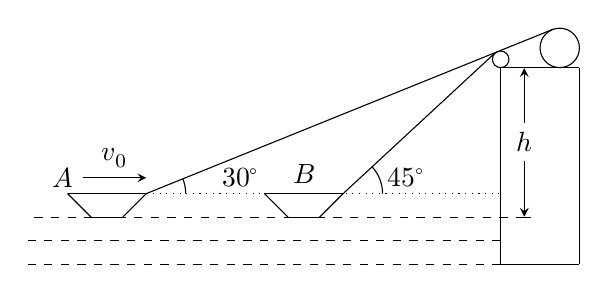
\begin{tikzpicture}[>=stealth]
			\draw[dashed] (0,0) to (-6,0);
			\draw[dashed] (0,0.3) to (-6,0.3);
			\draw[dashed] (0.3,0.6) to (-6,0.6);
			\draw (0,0) -- (0,2.5);
			\draw (0,0) -- (1,0);
			\draw (1,2.5) -- (1,0);
			\draw (1,2.5) -- (0,2.5);
			\begin{scope}[xshift=-5.5cm,yshift=0.9cm]
				\draw (0,0) to (1,0);
				\draw (0.3,-0.3) to (0,0);
				\draw (0.7,-0.3) to (1,0);
				\draw (0.7,-0.3) to (0.3,-0.3);
				\draw[->] (0.2,0.2)node[left]{$ A$}--node[above]{$ v_0 $}(1,0.2);
			\end{scope}
			\begin{scope}[xshift=-4.5cm,yshift=0.9cm]
				\draw (0,0) to (22:5.58);
				\draw[dotted] (0,0) to (0:4.5);
				\draw (0.5,0) arc (0:22:0.5);
				\node at (1.2,0.2) {$ 30^\circ $};
			\end{scope}	
			\begin{scope}[xshift=-3cm,yshift=0.9cm]
				\draw (0,0)--node[above]{$ B $} (1,0);
				\draw (0.3,-0.3) to (0,0);
				\draw (0.7,-0.3) to (1,0);
				\draw (0.7,-0.3) to (0.3,-0.3);
			\end{scope}
			\begin{scope}[xshift=-2cm,yshift=0.9cm]
				\draw (0,0) to (42.8:2.625);
				\draw (0.5,0) arc (0:42.8:0.5);
				\node at (0.8,0.2) {$ 45^\circ $};
			\end{scope}
			\draw (0.75,2.75) circle (0.25);
			\draw (0,2.605) circle (0.105);
			\draw[|<->|]  (0.3,0.5925) --node[fill=white]{$ h $} (0.3,2.5075);
		\end{tikzpicture}	
	}
	\subsubsection{T4}\noindent
	如图所示,一个质量为\,\SI{40}{kg}\,的小男孩站在一块放在水平地面的木板上,他发现鞋底与木板之间的动摩擦因数$ \mu_1 $比木板与地面之间的动摩擦因数$ \mu_2 $大一些,于是他尝试站在木板上,仅通过前后扭动身体实现木板的短距离移动. 假设男孩的重心仅在水平方向上移动,以向右的方向为$ x $轴的正方向,鞋底与木板间的最大静摩擦力为\,\SI{200}{N},木板与地面间的最大静摩擦力为\,\SI{50}{N},取重力加速度$ g=\SI{10}{m/s^2} $,为了让在男孩一次扭动身体后使木板实现向$ x $轴正方向移动一段距离,男孩的重心可以以下列哪种方式移动\\
	\begin{figure}[htp]
		\centering
		\begin{tikzpicture}[>=stealth]
			\draw[->] (0,0)node[left]{$ O $} to (90:2)node[right]{$ v /$\si{m.s^{-1}}};
			\draw[->] (0,0) -- (0:4) node[above] {$ t /$\si{s}} ;%坐标系ACD通用
			\draw (0,0) to (0.6,1);
			\draw (3,0)node[below]{1} to (0.6,1);%实线
			\draw[dashed] (0,1)node[left]{0.6} to (0.6,1);
			\draw[dashed] (0.6,0)node[below]{0.2} to (0.6,1);
			\node at (2,-0.75) {A};
			\begin{scope}[yshift=-4cm,xshift=0cm]
				\draw[->] (0,0)node[left]{$ O $} to (90:2)node[right]{$ v /$\si{m.s^{-1}}};
				\draw[->] (0,0) -- (0:4) node[above] {$ t /$\si{s}} ;%坐标系ACD通用
				\draw (0,0) to (2.4,1);
				\draw (3,0)node[below]{1} to (2.4,1);%实线
				\draw[dashed] (0,1)node[left]{0.6} to (2.4,1);
				\draw[dashed] (2.4,0)node[below]{0.8} to (2.4,1);
				\node at (2,-0.75) {C};
			\end{scope}
			\begin{scope}[yshift=-4cm,xshift=6cm]
				\draw[->] (0,0)node[left]{$ O $} to (90:2)node[right]{$ v /$\si{m.s^{-1}}};
				\draw[->] (0,0) -- (0:4) node[above] {$ t /$\si{s}} ;%坐标系ACD通用
				\draw (0,0) to (1.5,1);
				\draw (3,0)node[below]{1} to (1.5,1);%实线
				\draw[dashed] (0,1)node[left]{0.6} to (1.5,1);
				\draw[dashed] (1.5,0)node[below]{0.5} to (1.5,1);
				\node at (2,-0.75) {D};
			\end{scope}
			\begin{scope}[yshift=0cm,xshift=6cm]
				\draw[->] (0,0) to (90:2)node[right]{$ v /$\si{m.s^{-1}}};
				\draw[->] (0,1.3)node[left]{$ O $} -- (4,1.3) node[below] {$ t /$\si{s}} ;%坐标系ACD通用
				\draw (0,1.3) to (0.6,0.3);
				\draw (3,1.3)node[above]{1} to (0.6,0.3);
				\draw[dashed] (0,0.3)node[left]{$ -0.6 $} to (0.6,0.3);
				\draw[dashed] (0.6,1.3)node[above]{0.2} to (0.6,0.3);
				\node at (2,-0.75) {B};
			\end{scope}
			\begin{scope}[yshift=-1.75cm,xshift=12cm]
				\draw (0,0) to (4,0);
				\draw (1,0) to (3,0)to (3,0.2)to (1,0.2)--(1,0) ;
				\draw (1.5,0.2) to (2,0.7)to (2.5,0.2) to (2,0.7)--(2,1.2) ;
				\draw (1.6,0.8) to (2,1.2)to (2.4,0.8);
				\draw (2,1.4) circle (0.2);
			\end{scope}
		\end{tikzpicture}
	\end{figure}
	\clearpage\section{第三周}
	\subsection{星期一}\label{31}%杨子豪
	\noindent 如图\ref{31}\,所示,有一半导体砷化镓发光管发出波长为\:\SI{0.9}{\upmu m}的红外光,发光区为直径$ AB =\SI{3}{mm}$的圆盘,发光面上覆盖一折射率$ n=3.4 $的半球形介质. 若使发光区发出的全部光线在球面上都不发生全反射,介质半球的半径$ R $至少应该多大?
	\textfigure[figure-hsep=13.5cm]{}{
		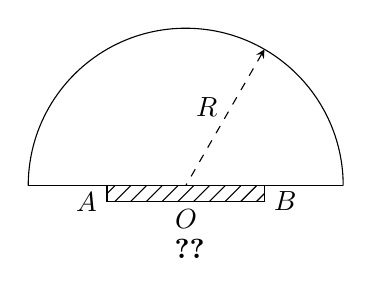
\begin{tikzpicture}[>=stealth]
			\draw (2,0) arc (0:180:2);
			\draw[dashed,<-] (60:2)--(0,0)node[below=.175cm]{$ O $};
			\begin{scope}[xshift=2cm]
				\node at (150:2){$ R $};
			\end{scope}
			\draw (-2,0)--(2,0);
			\draw (-1,0)--(-1,{-0.2})node[left]{$ A $}--node[below=.35cm]{图\ref{31}}(1,-0.2)node[right]{$ B $}--(1,0);
			\foreach \x in {-.7,-.5,...,.9}
			\draw (\x,0) --({\x-0.2},-0.2);
			\draw (-.9,0)--(-1,-0.1);
			\draw (1,-.1)--(.9,-0.2);
	\end{tikzpicture}}
	\\\,\\\,\\\,\\\,
	\subsection{星期二}%祝赫
	%答案:$ \dfrac{4\sqrt{3}}{3} $
	\noindent 已知椭圆$ \dfrac{x^2}{a_1^2}+\dfrac{y^2}{b_1^2}=1\,(a_1>b_1>0)$的离心率为$ e_1 $,双曲线$ \dfrac{x^2}{a_2^2}-\dfrac{y^2}{b_2^2}=1\,(a_1>0,b_1>0)$的离心率为$ e_2 $,二者共焦点$ F_1,F_2 $,在第一象限的交点$ P $满足$ \angle F_1PF_2=60^\circ $,则$ \dfrac{1}{e_1} +\dfrac{1}{e_2}$的最大值为\,\underline{\qquad\qquad}.
	\\\,\\\,\\\,\\\,\\\,
	\subsection{星期三}%乔冠嘉
	\noindent %答案:(1):$ \dfrac{5}{4} $;(2):$ -\dfrac{1}{1024} $.
	求下列各式的值:\\(1)\,$ \left(1+\cos\dfrac{\pi}{5}\right)\left(1+\cos\dfrac{3\pi}{5}\right) $;\\(2)\,\,$ \cos\dfrac{\pi}{11}\cos\dfrac{2\pi}{11}\cos\dfrac{3\pi}{11}\cdots\cos\dfrac{10\pi}{11}$.
	\clearpage \subsection{星期四}%孙晨惜
	\label{341}%$ x_R=-3 $
	\noindent
	$ P $为圆$ A:(x+2)^2+y^2=36 $上一动点,点$ B $的坐标为$ (2,0) $,线段$ PB $的垂直平分线交直线$ AP $于点$ Q $.\\
	(1)求点$ Q $的轨迹方程$ C $;
	\\(2)如图\ref{341},曲线$ C $与$ x $轴的两个交点分别为$ A_1,A_2$,$ M,N $为曲线$ C $上异于$ A_1,A_2$的两点,直线$ MN $不过原点,且不与坐标轴平行. 点$ M $关于原点$ O $的对称点为$ S $,若直线$ A_1S $与直线$ A_2N $相交于点$ T $,直线$ OT $与直线$ MN $相交于点$ R $.
	\textfigure[figure-hsep=-75pt,text-width=500pt,figure-vsep=0pt]{\noindent 求证:在曲线上存在定点$ E $使得$ \triangle RBE $的面积为定值,并求出该定值.
	}{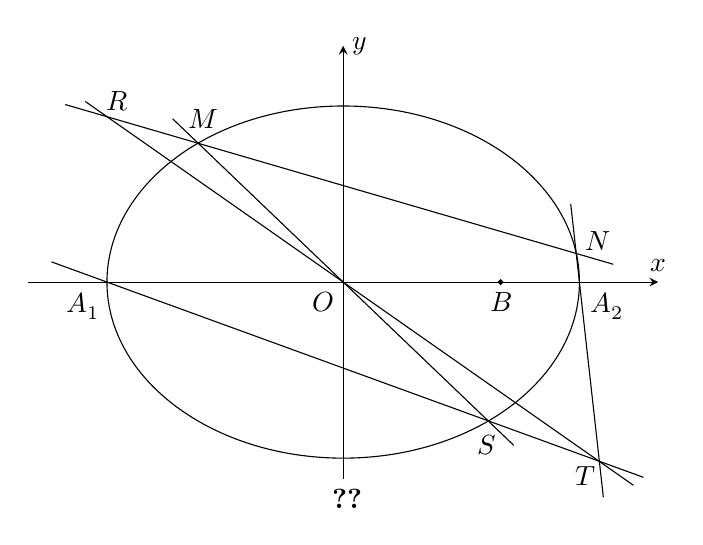
\begin{tikzpicture}[>=stealth]
			\draw[->] (-4,0)--(4,0)node[above] {$ x $};
			\draw[->] (0,-2.5)node[below]{图\ref{341}}--(0,3)node[right] {$ y $};
			\node at (-0.25,-.25) {$ O $};
			\draw[thick] (2,0)node[below]{$ B $} circle (0.02);
			\draw (0,0) ellipse (3 and {sqrt(5)});
			\draw (136.25:3)node[right=0.075cm]{$ M$}--(-43.75:3)node[left=0.12cm]{$ S$};
			\draw (145:4)node[right=0.15cm]{$ R $}--(-35:4.5);
			\begin{scope}[xshift=-3cm]
				\draw (160:0.75)--(-20:7.25);
				\node at (-0.3,-0.3) {$ A_1 $};
			\end{scope}
			\begin{scope}[xshift=3cm]
				\draw (96.35:1)--(-83.65:2.75)node[left=0.25cm,above=0.02cm]{$ T $};
				\node at (0.35,-0.3) {$ A_2 $};
			\end{scope}
			\begin{scope}[xshift=-1.85cm,yshift=1.765cm]
				\draw (180-16.25:1.75)--(-16.25:5.5)node[above=0.3cm,left=-.05cm]{$ N $};
			\end{scope}
	\end{tikzpicture}}
	\\\,
	\subsection{星期五:随机抽,请各位做好准备}%随机抽
	\label{321}%答案:D
	\noindent 将一个半球体置于水平地面上,半球的中央有一光滑小孔,上端有一光滑的小滑轮,柔软光滑的轻绳绕过滑轮,两端分别系有质量为$ m_1,m_2 $的小球$ A,B $(两小球均体积不计,可看成质点,$ B $悬于空中)时,整个装置处于静止状态,如图\ref{321}\,所示. 已知此时$ A $与半球的球心$ O $的连线与水平方向成$ \alpha $角($\sin\alpha=0.6,\cos\alpha=0.8 $),$ A $与半球间的动摩擦因数$\mu=0.5  $,$  A$所受到的最大静摩擦力等于滑动摩擦力. 则在整个装置处于静止的情况下,下列说法正确的是
	\textfigure[figure-hsep=15pt,figure-vsep=0pt]{
		\setlength{\lineskip}{8pt}
		\setlength{\lineskiplimit}{8pt}
		\noindent A.\,当$ \dfrac{m_1}{m_2} $不同时,地面对半球体的摩擦力也不同
		\\B.\,半球体对$ A $的支持力随$ B $的质量$ m_2 $变化而变化
		\\C.\,随着$ B $的质量$ m_2 $增大,$ A $所受半球体的摩擦力一定增大
		\\D.\,当$ \dfrac{5}{4}<\dfrac{m_1}{m_2}\le2 $时,半球体对$ A $的摩擦力的方向垂直图中的虚线向上
	}{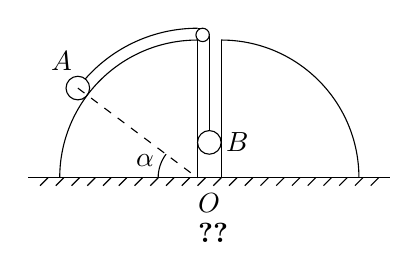
\begin{tikzpicture}
			\draw (0,0.45)node[right=0.1cm]{$ B $} circle (0.15);
			\draw (-2.3,0)--(2.3,0);
			\draw (-0.15,0)--(-0.15,1.75);
			\draw (0.15,0)--(0.15,1.75);
			\draw (-0.15,1.75) arc (90:180:1.75);
			\draw (0.15,1.75) arc (90:0:1.75);
			\draw (-1.67,1.14)node[left=0.2cm,above=0.1cm]{$ A $} circle (0.15);
			\draw[dashed]  (-1.67,1.14)--(-0.15,0) ;
			\draw (-0.65,0) arc (180:{180-37}:0.5);
			\node at (0,-0.325) {$ O $};
			\node at (0,-0.7) {图\ref{321}};
			\begin{scope}[xshift=-0.15cm]
				\node at (162:0.7) {$ \alpha $};
				\draw (0,1.9) arc (90:138.75:1.9);
				\draw (0,1.9) --(0.075,1.9);
			\end{scope}
			\draw (-0.085,1.815) circle (0.085);
			\draw (0,0.6) --(90:1.7957);
			\foreach \x in {-2.05,-1.85,...,2.15}
			\draw (\x,0)--({\x-0.1},-0.1);
	\end{tikzpicture}}
	\clearpage\section{第四周}
	\subsection{星期一}\label{41}\noindent%徐博达
	二元酸$ \ce{H_2A} $在水中有如下的解离方式:
	\begin{align*}
		\ce{H_2A &<=> H^+ + HA-}\qquad K_{\mathrm{a}1},
		\\\ce{HA- &<=> H^+ + A^{2-}}\qquad\:\, K_{\mathrm{a}2}.
	\end{align*}(1)可以通过计算认为$ \ce{H_2A} $等粒子的浓度只与氢离子的浓度有关,例如:\begin{empheq}[box = \fbox]{align*}
		c(\mathrm{H_2A})&=\dfrac{c(\mathrm{H_2A})}{c(\mathrm{H_2A})+c(\mathrm{HA^-})+c(\mathrm{A^{2-}})}c_0
		\text{\qquad 根据物料守恒:$ c_0=c(\mathrm{H_2A})+c(\mathrm{HA^-})+c(\mathrm{A^{2-}})$是常值}
		\\&=\dfrac{1}
		{1+\dfrac{c(\mathrm{HA^-})}{c(\mathrm{H_2A})}+\dfrac{c(\mathrm{A^{2-}})}{c(\mathrm{H_2A})}}c_0
		\\&=\dfrac{1}
		{1+\dfrac{K_{\mathrm{a}1}}{c(\mathrm{H^+})}+\dfrac{K_{\mathrm{a}1}K_{\mathrm{a}2}}{c^2(\mathrm{H^+})}}c_0
		=\dfrac{c^2(\mathrm{H^+})}
		{c^2(\mathrm{H^+})+K_{\mathrm{a}1}c(\mathrm{H^+})+K_{\mathrm{a}1}K_{\mathrm{a}2}}c_0.
	\end{empheq}
	根据上述推导,试求出$ c(\mathrm{HA^-}),c(\mathrm{A^{2-}}) $与$  c(\mathrm{H^+})$的关系;
	\\(2)有时在我们考试时会看到如图\ref{41}\:来表示二元酸$ \ce{H_2A} $的分布系数(这里以$ \ce{H2C2O4} ,\SI{25}{\degreeCelsius}$为例):
	\begin{figure}[htp!]
		\centering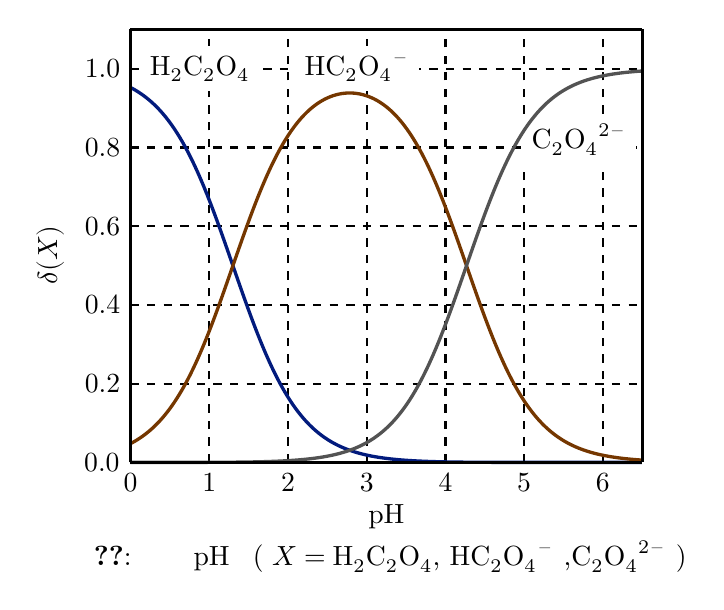
\begin{tikzpicture}[thick]	\draw[dashed](0,1)node[left]{0.2}--(6.5,1);
			\draw[dashed](0,2)node[left]{0.4}--(6.5,2);
			\draw[dashed](0,3)node[left]{0.6}--(6.5,3);
			\draw[dashed](0,4)node[left]{0.8}--(6.5,4);
			\draw[dashed](0,5)node[left]{1.0}--(6.5,5);
			\draw[dashed] (1,0)node[below]{1}--(1,5.5);
			\draw[dashed] (2,0)node[below]{2}--(2,5.5);
			\draw[dashed] (3,0)node[below]{3}--(3,5.5);
			\draw[dashed] (4,0)node[below]{4}--(4,5.5);
			\draw[dashed] (5,0)node[below]{5}--(5,5.5);
			\draw[dashed] (6,0)node[below]{6}--(6,5.5);
			\node[fill=white] at (0.88,5) {\ce{H2C2O4}};
			\node[fill=white] at (2.88,5) {\ce{HC2O4^-}};
			\node[fill=white] at (5.7,4.1) {\ce{C2O4^{2-}}};
			\definecolor{cn}{RGB}{2,27,125};
			\definecolor{cnm}{RGB}{117,55,0};
			\definecolor{cm}{RGB}{83,83,83};
			\draw[smooth,domain=0:6.5,samples=650,color=cn,very thick]
			plot(\x,\fpeval{5/(1+0.05*10^{\x}+0.05*0.000054*100^{\x})});
			\draw[smooth,domain=0:6.5,samples=650,color=cnm,very thick]
			plot(\x,\fpeval{5/(1+10^{-\x}/0.05+0.000054*10^{\x})});
			\draw[smooth,domain=0:6.5,samples=650,color=cm,very thick]
			plot(\x,\fpeval{5/(1+100^{-\x}/0.05/0.000054+10^{-\x}/0.000054)});
			\draw[very thick] (0,0)node[below]{0}--node[left=0.7cm,above=-0.12cm,rotate=90]{$ \delta(X)$}(0,5.5);
			\draw[very thick] (0,0)node[left]{0.0}--node[below=0.4cm]{pH}(6.5,0);
			\draw[very thick] (6.5,0)--(6.5,5.5);
			\draw[very thick] (0,5.5)--(6.5,5.5);
			\node at (13/4,-1.2) {图\ref{41}:草酸的分布系数随pH的变化( $X=$\:\ce{H2C2O4}, \ce{HC2O4^-} ,\ce{C2O4^{2-}} )};
		\end{tikzpicture}
	\end{figure}\\我们发现一个规律:\:\ce{H_2A}线与\:\ce{A^{2-}}线交点与\:\ce{HA-}线最高点对应的pH相等. 试证明此规律.
	\clearpage\subsection{星期二}\label{42}\noindent%答案:(1)$ n=\sqrt{3}$;(2)$ d>\dfrac{\sqrt{3}}{6}a $
	如图\ref{42}\:所示为某种透明材料做成的三棱镜,其横截面是边长为$ a $的等边三角形$ ABC $,现用一束宽度为$ a $的单色平行光束,以垂直于$ BC $面的方向入射到该三棱镜的$ AB $及$ AC $面上,结果所有从$ AB,AC $面入射的光线进入后恰好全部直接到达$ BC $面. 
	\textfigure[]{\setlength{\lineskip}{8pt}
		\setlength{\lineskiplimit}{8pt}\noindent(1)求该材料对此平行光束的折射率$ n $;
		\\(2)这些直接到达$ BC $面的光线从$ BC $面折射而出后,如果照射到一块平行于$ BC $面的屏$ \alpha $上形成光斑,若此光斑分为两块,求屏$ \alpha $到$ BC $面的距离$ d $的取值范围.}{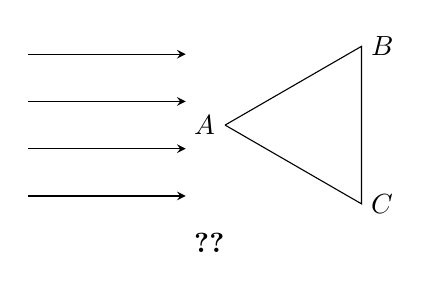
\begin{tikzpicture}[>=stealth]
			\foreach \x in {-.9,-.3,...,.9}
			\draw[->] (-2.5,\x)--(-.5,\x);
			\draw (0,0)node[left]{$ A $}--(30:2)node[right]{$ B $}--(-30:2)node[right]{$ C $}--(0,0);
			\node at (-.25,-1.5) {图\ref{42}};
	\end{tikzpicture}}
	\\\,\\\,\\\,\\\,\\\,\\\,
	\subsection{星期三}
	\subsubsection{T1}\label{431}\noindent
	如图\ref{431}\:所示,在$ O $点固定一个正电点电荷. 同时在以$ O $为圆心,$ \dfrac{1}{2}a $为半径的虚线圈有垂直纸面向里的匀强磁场(图中未画出),$ MSN $是由细管制成的半径为$ a $的光滑绝缘圆轨道,其圆心位于$ O $点. 在$ M $点以速度$ v_0 $垂直$ MN $向下射出一个质量为$ m $(不计重力),电荷量为$ q $的负电粒子,粒子恰好做匀速圆周运动,从$ N $点进入圆轨道(细管的内径略比粒子大). 粒子从$ N $点进入后开始计时,虚线圆内磁场的磁感应强度按$ B=B_0-\beta t\,(\beta>0) $的规律开始变化,粒子从$ M $点出来时磁感应强度的大小恰好变为0,之后不再变化,此时撤去圆轨道,粒子轨迹变为椭圆且垂直穿过$ MN $线上的$ P $点,$ OP=7a $. 若以无穷远为零电势,则点电荷电场中某点的电势$ \varphi=\dfrac{kQ}{r}$,其中$  k$为静电力常量,$ Q $为点电荷带电量,$ r $为某点到点电荷的距离. 求:
	\textfigure{\setlength{\lineskip}{8pt}
		\setlength{\lineskiplimit}{8pt}
		\noindent(1)固定在$ O $点的正电点电荷的电荷量$ Q $;
		\\(2)虚线圆内磁场初磁感应强度$ B_0 $与其变化率的绝对值$ \beta $;
		\\(3)粒子从出发到达$ P $点的时间$ t $.
	}{\begin{tikzpicture}[>=stealth]
			\draw[dashed] (-3.5,0)--(3.5,0);
			\draw[dashed] (0,0) circle (.7);
			\draw (1.4,0)node[below]{$ N $} arc (0:180:1.4);
			\draw (1.5,0) arc (0:180:1.5);
			\draw[->] (-1.45,-.1) --node[right]{$ v_0 $}(-1.45,-.7);
			\node at (3.3,-.25) {$ P $};
			\node at (0,1.75) {$ S $};
			\node at (-1.75,.25) {$M $};
			\node at (0,-1.1) {图\ref{431}};
			\draw (0,0) circle (.1);
			\draw (-.1,0) -- (.1,0);
			\draw (0,-.1) -- (0,.1);
			\node at (-.2,.2) {$ O $};
	\end{tikzpicture}}
	\clearpage\subsubsection{T2}\label{432}\noindent
	如图\ref{432}\:所示,$ ABCD-A'B'C'D' $为一厚度$ OO'=L $,折射率$ n=\frac{\sqrt{6}}{2} $的“回”字形固定正方体玻璃砖截面,$ OO' \perp AD $,且$ AO=OD , A'D'=4L ,AD=6L$,一束单色光$ PO $沿与$ OO' $成$ θ=60^\circ $的方向射向$ O $点经折射后打到$ A'D' $边上,$ A'B',B'C',CD,OD $(不包括$ O $点)均涂有特殊材料,其使光在该表面不发生反射和折射,足够大的光屏$ MN $紧靠在玻璃砖的右侧. 求$ MN $上两光点的距离.
	\textfigure[text-width=13cm,figure-hsep=13cm]{}{\begin{tikzpicture}[>=stealth]
			\foreach \x in {1,1.5}
			\draw (45:\x)--(135:\x)--(225:\x)--(-45:\x)--(45:\x);
			\node at (45:0.7) {$ D' $};
			\node at (135:0.68) {$ A' $};
			\node at (225:0.68) {$ B' $};
			\node at (-45:0.7) {$ C' $};
			\node at (45:1.8) {$ D $};
			\node at (135:1.8) {$ A $};
			\node at (225:1.8) {$ B $};
			\node at (-45:1.8) {$ C $};
			\node at (.275,.875) {$ O'$};
			\node at (.25,1.25) {$ O $};
			\begin{scope}[xshift=0pt,yshift=\fpeval{sqrt(1.125)}cm]
				\draw[->](150:2)node[above]{$ P $}--(150:1);
				\draw(150:2)--(150:0);
				\draw (0,0.3) arc (90:150:0.3);
				\node at (120:0.5) {$ \theta $};
			\end{scope}
			\draw[dashed] (0,3) -- (0,-3);
			\begin{scope}[yshift=0pt,xshift=\fpeval{sqrt(1.125)}cm]
				\draw[dashed] (0,3.5)node[right]{$ M $} -- (0,-3.5)node[right]{$ N $};
			\end{scope}
			\node at (0,-3.9){图\ref{432}};
	\end{tikzpicture}}
	\subsection{星期四}
	\subsubsection{T1}\noindent%答案$ a_n=\dfrac{1}{2^n}+\dfrac{1}{n(n+1)} $
	已知数列$ \{a_n\} $的首项$ a_1=1 $,且满足$ 2a_{n+1}-a_n=\dfrac{n-2}{n(n+1)(n+2)} $,则数列$ \{a_n\} $的通项公式为\:\underline{\qquad\qquad}.
	\\\,\\\,
	\subsubsection{T2}\noindent%答案$ a_n=2^{2^{n-1}}-1 $
	已知数列$ \{a_n\} $的首项$ a_1=1 $,且满足$ a_{n+1}=2a_n^2$,则数列$ \{a_n\} $的通项公式为\:\underline{\qquad\qquad}.
	\\\,\\\,
	\subsection{星期五:随机抽,请各位做好准备}\noindent%答案:$ \dfrac{61}{243} $
	春节到了,祝赫,杜念龙,张煜绅,邱琳琳发红包,规定每个人发的红包自己不能抢,手气最佳发下一轮. 若祝赫发第一个红包,求第七个红包仍是祝赫发的概率. 
	\clearpage\section{第五周}
	\subsection{星期一}\noindent
	已知数列$ \{a_n\} $的前$ n $项和为$ S_n $,首项$ a_1=2 $,满足$ a_n+2n=2a_{n-1}+4\:(n\ge2) $,数列$ \{b_n\} $的通项$ b_n=\dfrac{S_n}{n} $,则使得$ \dfrac{1}{b_1^2}+\dfrac{1}{b_2^2}+\cdots+\dfrac{1}{b_n^2}<k $恒成立的最小的$ k $值最接近\begin{xchoices}[label-style=Alph]
		\item $ \dfrac{1}{2} $
		\item $ \dfrac{7}{10} $
		\item $ \dfrac{3}{4} $
		\item $ 1 $
	\end{xchoices}\\\quad\\\quad\\\quad\\\quad\\\quad\\\quad
	\subsection{星期二}\noindent
	在以下条件下,求数列$ \{a_n\} $的通项公式:
	\\(1)\:$ a_1=1 $,递推公式为$ a_{n+1}=2a_n-1 $;\\\,\\\,\\\,\\\,
	\\(2)\:$ a_1=1,a_2=2 $,递推公式为$ a_{n+2}=2a_{n+1}-a_n $;\\\,\\\,\\\,\\\,
	\\(3)\:$ a_1=a_2=1$,递推公式为$ a_{n+2}=a_{n+1}+a_n $;\\\,\\\,\\\,\\\,
	\\(4)\:$ a_1=a_2=1, a_3=2$,递推公式为$ 3a_{n+3}=4a_{n+2}+a_{n+1}-2a_n $.
	\clearpage\subsection{星期三}\noindent
	将$ n^2 $个正实数排成$ n $行$ n $列:
	\begin{align*}
		\begin{matrix}
			a_{11} & a_{12} & \cdots & a_{1n}\\
			a_{21} & a_{22} & \cdots & a_{2n}\\
			\cdots & \cdots & \cdots & \cdots\\
			a_{n1} & a_{n2} & \cdots & a_{nn}\\
		\end{matrix},
	\end{align*}其中每一行的数成等差数列,每一列的数成等比数列,且所有的公比相等.
	\\已知$ a_{24}=1 ,a_{42}=\dfrac{1}{8},a_{43}=\dfrac{3}{16}$. 求$ a_{11}+a_{22}+\cdots+a_{nn} $的值.
	\\\,\\\,\\\,\\\,\\\,
	\subsection{星期四}\noindent
	已知数列$ \{a_n\} $满足$ a_1=1 $,$ a_{n+1}=\dfrac{n^2+n+1}{n^2+n}a_n+\dfrac{1}{2^n} $.
	\\(1)求证:当$ n\ge2 $时,$ a_n\ge2 $;
	\\(2)求证:$ a_{n+1}=\dfrac{1}{1\cdot2}a_1+\dfrac{1}{2\cdot3}a_2+\cdots+\dfrac{1}{n\cdot(n+1)}a_n+2-\dfrac{1}{2^n} $;
	\\(3)已知若$ x>-1 $,则$ \ln(1+x)<x $恒成立. 求证:$ a_n<\dfrac{43}{12}\sqrt{\eu}-1 $.\\\,\\\,\\\,\\\,\\\,\\\,
	\subsection{星期五:随机抽}\noindent
	已知椭圆$ \varGamma:\dfrac{x^2}{4}+\dfrac{y^2}{3}=1 $,过其左焦点$ F_1 $做直线$ l $交椭圆$ \varGamma $于$ A,P $两点,取点$ P $关于$ x $轴的对称点$ B $,若$ G $为$ \triangle PAB $的外心,则$ \dfrac{|PA|}{|GF_1|} $的值为
	\begin{xchoices}[label-style= Alph]
		\item 2
		\item 3
		\item 4
		\item 以上都不对
	\end{xchoices}
	\clearpage\section{第六周}
	\subsection{星期三}\noindent
	《缀术》是中国南北朝时期的一部算经,汇集了祖冲之和祖暅父子的研究成果. 《缀术》中提出的“原幂势既同,则积不容异”被称为祖暅原理,其意思是:如果两等高的几何体在同高处被截得的两截面面积均相等,那么这两个几何体的体积相等. 该原理常应用于计算某些几何体的体积. 根据以上信息,回答下列问题. 
	\subsubsection{T1}\label{611}\textfigure[text-width=18cm, fig-pos = bottom-center]{
		\noindent
		如图\:\ref{611},某个西晋越窑卧足杯的上下底为互相平行的圆面,侧面为球面的一部分,上底直径为$ 4\sqrt{6}\,\si{cm} $,下底直径为\:\SI{6}{cm},上下底间的距离为\:\SI{3}{cm},则该卧足杯侧面所在的球面的半径是\:\underline{\qquad\qquad}\,\si{cm};卧足杯的容积是\:\underline{\qquad\qquad}\,\si{cm^3}\:(杯的厚度忽略不计).}{
		\begin{tikzpicture}
			\centering
			\node at (0,0) {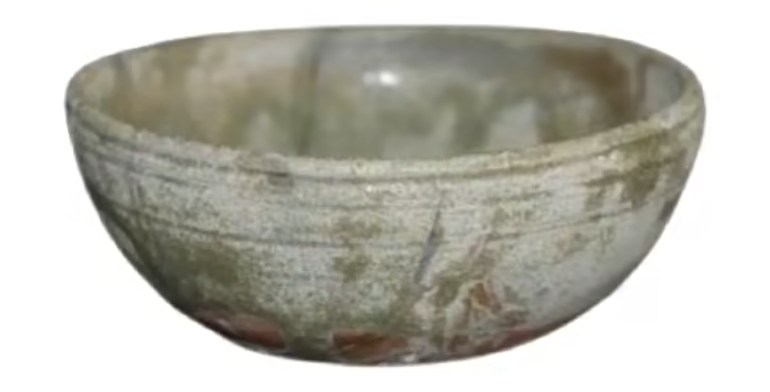
\includegraphics[width=6cm]{611.png}};
			\node at (0,-2) {图\:\ref{611}};
	\end{tikzpicture}}
	\subsubsection{T2}\label{612}\noindent
	如图\:\ref{612},在$ xOy$平面上将两个半圆弧$ (x-1)^2+y^2=1\:(x\ge1) $与$ (x-3)^2+y^2=1\:(x\ge3) $,两条直线$ y=1 $与$ y=-1 $围成的封闭图形记为$ D $即图中阴影部分. 记$ D $绕$ y $轴旋转一周而成的几何体为$ \Omega $,过点$ (0,y)\:(|y|\le1) $作$ \Omega $的水平截面,所得截面面积为$ 4\pi\sqrt{1-y^2}+8\pi $,则$ \Omega $的体积为\:\underline{\qquad\qquad}.\textfigure[figure-hsep=11cm]{}{
		\begin{tikzpicture}[>=stealth]
			\definecolor{grey}{RGB}{195,195,195}
			\filldraw[grey,linewidth=0cm] (1,1)--(3,1)--(3,-1)--(1,-1)--(1,1);
			\filldraw[white] (1,1) arc (90:-90:1);
				\filldraw[grey] (3,1) arc (90:-90:1);
			\filldraw[white] (1,0) circle (1);
			\draw[grey] (3,1)--(3,-1);
			\draw[->](-.7,0)--(4.7,0)node[below]{$ x $};
			\draw[->](0,-1.7)--(0,1.7)node[left]{$ y $};
			\node at (-.3,-.3) {$O  $};
			\foreach \x in {1,2,...,4}{
				\draw[thick] (\x,0) circle (1/50);
				\node at (\x,-.3) {\x};	
			}
			\foreach \y in {-1,1}{
				\node at (-.3,\y) {$ \y $};	
				\draw[thick] (0,\y) circle (1/50);
				\draw (1,\y) -- (3,\y);
			}
			\foreach \t in {1,3}{
				\draw (\t,1) arc (90:-90:1);
			}
			\node at (2.5,.5) {$ D $};
			\node at (2,-2) {图\:\ref{612}};
	\end{tikzpicture}}
	\\\,
	\\\,
	\\\,\\	
	祝同学们阶段考试顺利!
	\clearpage\section{第七周}
	\subsection{星期三}
	\subsubsection{T1}\noindent
	设数列$ \{a_n\} $的前$ n $项和为$ S_n $,且$ a_n=\sqrt{n\cdot(n+1)} $.
	\\求证:$ \dfrac{n(n+1)}{2}<S_n<\dfrac{n(n+2)}{2} $.
	\\\,\\\,
	\subsubsection{T2}\noindent
	设数列$ \{a_n\} $满足$ a_{n+1}=a_n^2-na_n+1 $,且$ a_n\ge n+2 $,且数列$ \left\{\dfrac{1}{a_n+1}\right\} $的前$ n $项和为$ S_n $.
	\\求证:$ S_n<\dfrac{1}{2} $.
	\\\,\\\,
	\subsubsection{T3}\noindent
	设数列$ \{a_n\} $的前$ n $项积为$ T_n $,且$ a_n=\dfrac{2n-1}{2n} $.
	\\求证:$ T_n<\sqrt{\dfrac{1}{2n+1}} $.
	\\\,\\\,
	\subsubsection{T4}\noindent
	设数列$ \{a_n\} $的通项$ a_n=\left(1+\dfrac{1}{2n}\right)^n $.
	\\求证:$ \dfrac{3}{2}\le a_n<2 $.
	\\\,\\\,
	\subsection{星期四}\noindent
	已知等比数列$ \{a_n\} $的前$ n $项和为$ S_n $,点$ (n,S_n) $均在曲线$ y=b^x+r\,(\:b>0\:\text{且}\:b\ne1\text{,}b,r\:\text{均为常数}) $上.
	\\(1)求$ r $的值;
	\\(2)当$ b=2 $时,记$ c_n=2(\log_2a_n+1) $. 
	\\求证:$ \forall n\in\mathbb{N^*} $,均有$ \dfrac{c_1+1}{c_1}\cdot\dfrac{c_2+1}{c_2}\cdots\dfrac{c_n+1}{c_n}>\sqrt{n+1} $成立.
	\section{第八周}
	\subsection{星期一06}\noindent
	(多选)已知数列$ \{a_n\} $的通项$ a_n=\dfrac{1}{n} $,其前$ n $项和为$ S_n $. $ b_n=\dfrac{\ln(1+a_n)}{a_n} $,则下列说法正确的是\begin{xchoices}[label-style=Alph]
		\item $ a_{n+1}<\ln\dfrac{n+1}{n}<a_n $
		\item 数列$ \{b_n\} $是递增数列
		\item $ S_{2021}-1>\ln2021>S_{2020} $
		\item $ \ln2\le b_n<\ln3 $
	\end{xchoices}\noindent
	参考条件:当$ x>0
	 $时,$ \ln(1+x)<x $恒成立.
	\\\,\\\,\\\,\\\,
	\subsection{星期二44}\label{82}\noindent
	\textfigure[figure-hsep=.35 cm]{\setlength{\lineskip}{8pt}
		\setlength{\lineskiplimit}{8pt}\noindent
		直立的汽缸内装有一定质量的理想气体,其满足理想气体状态方程$ pV=nRT $,单位物质的量这种气体的内能$ E=\dfrac{3}{2}RT $,其中$ R $为摩尔气体常数,$ T $为热力学温度,$ p $为气体产生的压强,$ V $为气体体积. 
		\\质量$ M=7.00\,\si{kg} $的活塞与一劲度系数$ k=300\,\si{N/m} $的轻质弹簧相连,弹簧下端固定在气缸底部,如图\:\ref{82}\:所示. 活塞与气缸壁间的摩擦及弹簧的体积均忽略不计. 平衡时,测得缸内气体温度$ T_1=300\,\si{K} $,压强$ p_1=\SI{1.40e6}{Pa} $,气柱长$ L_1=\SI{50.0}{cm} $. 而活塞上方大气压强$ p_0=\SI{1.00e5}{Pa} $,活塞的截面积$ S=\SI{25.0}{cm^2} $. 
		\\现有一质量$ m=\SI{3.00}{kg} $的铅柱自活塞正上方高$ H=\SI{80.0}{cm}$处自由落下,与活塞发生完全非弹性碰撞,碰撞时间极短而可忽略. 已知碰后铅柱在运动过程中某一时刻又与活塞分开,此时气缸内的温度$ T_2=\SI{290}{K} $,铅柱最终上升到活塞初始位置上方$ h=\SI{7.80}{cm} $高处.
		\\试求自铅柱与活塞开始一起向下运动到铅柱刚离开活塞的整个过程中,外界传给气缸内气体的热量$ Q $.
		\\计算中重力加速度$ g $取\:\SI{10.0}{m/s^2},并假设活塞是绝热的,气缸壁是可以导热的,弹簧始终处于弹性限度之内.}{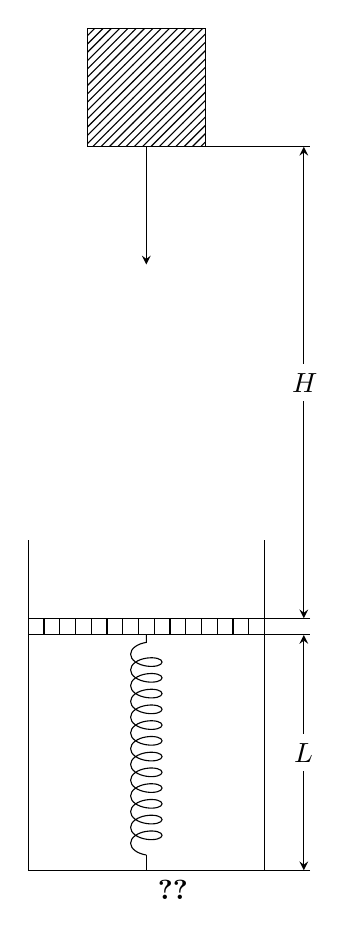
\begin{tikzpicture}[>=stealth]
			\draw[|<->|] (2,-19/2560)--node[fill=white]{$ L $}(2,{3+19/2560});
			\begin{scope}[yshift=3.2 cm]
				\draw[|<->|] (2,-19/2560)--node[fill=white]{$ H $}(2,{6+19/2560});
			\end{scope}
			\draw[decoration={aspect=0.5, segment length=2 mm, amplitude=2 mm,coil},decorate] (0,0.2) -- (0,3);
			\draw (0,0)--(0,.2);
			\draw (-1.5,0)--node[below]{图\:\ref{82}}(2,0);
			\draw (-1.5,3)--(2,3);
			\draw (-1.5,3.2)--(2,3.2);
			\draw (-1.5,4.2)--(-1.5,0);
			\draw (1.5,4.2)--(1.5,0);
			\foreach \x in {-1.3,-1.1,...,1.3}
			\draw (\x,3)--(\x,3.2);
			\begin{scope}[yshift=9.2 cm]
				\draw (0,0)--(2,0);
				\draw[->] (0,0)--(-90:1.5);
				\draw (-.75,0)--(.75,0)--(.75,1.5)--(-.75,1.5)--(-.75,0);
				\fill[pattern = north east lines,step=0.25cm] (-.75,0) rectangle (.75,1.5);
			\end{scope}
		\end{tikzpicture}
	}
	\clearpage
	\subsection{星期三39}\noindent
	已知数列$ \{a_n\} $的首项$ a_1=\dfrac{1}{2} $,且$ a_{n+1}=\dfrac{1}{3}a_n^3+\dfrac{2}{3}a_n $.
	\\求证:$ \dfrac{1}{2}\cdot\left(\dfrac{2}{3}\right)^{n-1}\le a_n\le\dfrac{1}{2}\cdot\left(\dfrac{3}{4}\right)^{n-1} $.
	\\\,\\\,\\\,\\\,\\\,\\\,\\\,\\\,\\\,
	\subsection{星期四54}\noindent
	已知数列$ \{a_n\} $的首项$ a_1=1 $,递推公式为$ a_{n+1}=\dfrac{a_n}{1+\sqrt{a_n}} $,前$ n $项和为$ S_n $,则下列说法正确的是\begin{xchoices}[label-style=Alph]
		\item $ \dfrac{3}{2}<S_{100}<3 $
		\item $ 3<S_{100}<4 $
		\item $ 4<S_{100}<\dfrac{9}{2} $
		\item $ \dfrac{9}{2}<S_{100}<5$
	\end{xchoices}
	\clearpage\section{第九周}
	\subsection{星期一26}\noindent
	已知函数$ f(x)=\ln x+ax^2+(2a+1)x $,其中$ a\in\mathbb{R} $.
	\\(1)讨论$ f(x) $的单调性;
	\\(2)当$ a<0 $时,求证:$ f(x)\le-\dfrac{8a+3}{4a} $
	\\\,\\\,\\\,\\\,\\\,\\\,\\\,\\\,\\\,\\\,\\\,\\\,
	\subsection{星期二51}\noindent
	已知函数$ f(x)=x^3-3x^2+5,g(x)=m(x+1) $. 若存在唯一的正整数$ x_0 $使得$ f(x_0)<g(x_0) $,则实数$ m $的取值范围为\begin{xchoices}[label-style=Alph]
		\item $ \left[0,\dfrac{5}{4}\right] $
		\item $ \left[\dfrac{1}{3},\dfrac{5}{4}\right] $
		\item $ \left(\dfrac{1}{3},\dfrac{5}{4}\right] $
		\item $ \left(0,\dfrac{1}{3}\right) $
	\end{xchoices}
	\clearpage\subsection{星期三21}\noindent
	已知正项数列$ \{a_n\} $的首项$ a_1=2 $,递推公式为$ (n+1)a_{n+1}^2=na_n^2+a_n $,则下列说法正确的是
	\begin{xchoices}[label-style=Alph]
		\item $ a_n^2\le\dfrac{2n+2}{n} $
		\item $ \dfrac{a_2^2}{2^2}+\dfrac{a_3^2}{3^2}+\dfrac{a_4^2}{4^2}+\cdots+\dfrac{a_n^2}{n^2}<2 $
		\item $ 1<a_{n+1}<a_n$
		\item $ 2\le a_{n}<a_{n+1} $
	\end{xchoices}
	\\\,\\\,\\\,\\\,\\\,\\\,\\\,\\\,\\\,\\\,\\\,
	\subsection{星期四03}
	\subsubsection{T1}\label{941}\noindent
	如图\:\ref{941},现有一圆柱形长管,长$ L=\SI{125}{cm} $,内盛有长$ l=\SI{25}{cm} $的汞柱,底部气柱高$ h=\SI{90}{cm} $. 已知大气压强$ p_0=\SI{75}{cmHg} $,初始温度$ T_0=\SI{270}{K} $. 现升高环境温度(不影响大气压强),求水银完全溢出时所需的最低温度$ T_{\min} $.
	\textfigure[fig-pos=right,text-width=16cm,figure-hsep=15cm]{}{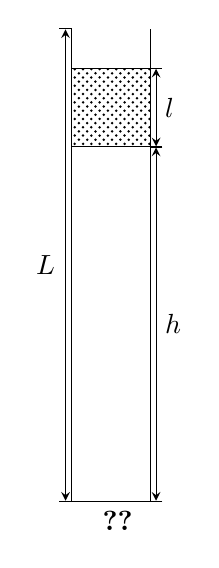
\begin{tikzpicture}[>=stealth]
			\draw[|<->|] (-.575,{6+19/2560})--node[left]{$ L $}(-.575,-19/2560);
			\draw[|<->|] (.575,{4.5+19/2560})--node[right]{$ h $}(.575,-19/2560);
			\draw[|<->|] (.575,{4.5-19/2560})--node[right]{$ l $}(.575,{5.5+19/2560});
			\draw (-.5,6)--(-.5,0)--node[below]{图\:\ref{941}}(.5,0)--(.5,6);
			\draw[pattern={crosshatch dots}] 
			(-.5,4.5) rectangle +(1,1);
	\end{tikzpicture}}
	\clearpage\subsubsection{T2}\label{942}\noindent
	(多选)如图\:\ref{942}\:所示,小球$ A,B $用一根长为$ L $的轻杆相连,竖直放置在光滑水平地面上,小球$ C $挨着小球$ B $放置在地面上. 由于微小扰动,小球$ A $沿光滑的竖直墙面下滑,小球$ B,C $在同一竖直面内向右运动. 当杆与墙面夹角为$ \theta $,小球$ A $与墙面恰好分离,最后小球$ A $落到水平地面上. 则下列说法正确的是
	\textfigure{\begin{xchoices}[label-style=Alph]
			\setlength{\lineskip}{8pt}
			\setlength{\lineskiplimit}{8pt}
			\item 当小球$ A $的机械能达到最小时,小球$ B $和小球$ C $的加速度为0
			\item 在小球$ A $由静止到与墙面分离的过程中,小球$ B $的速度先增大后减小
			\item 当小球$ A $与墙面恰好分离时,小球$ B $与小球$ C $也恰好分离
			\item 当小球$ A $与墙面恰好分离时,小球$ A $与小球$ B $的速度之比为$ \tan\theta:1 $
	\end{xchoices}}{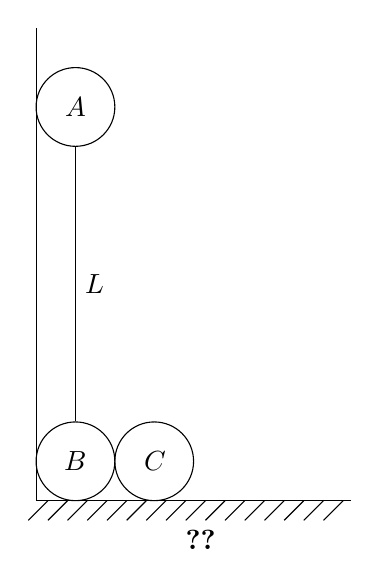
\begin{tikzpicture}
			\draw (0,6)--(0,0)--(4,0);
			\node[minimum width=1cm,
			minimum height=1cm,circle,draw=black](b) at (.5,.5){$ B $};
			\node[minimum width=1cm,
			minimum height=1cm,circle,draw=black](c) at (1.5,.5){$ C $};
			\node[minimum width=1cm,
			minimum height=1cm,circle,draw=black](a) at (.5,5){$ A $};
			\draw (a)--node[right]{$ L $}(b);
			\foreach \x in {.1,.35,...,3.85}
			\draw (\x+.05,0)-- +(-.25,-.25);
			\node at (2,-.50) {图\:\ref{942}};
	\end{tikzpicture}}\\思考题:在原基础上拿去小球$ C $,且小球$ A,B $质量相等. 当小球$ A $与墙面分离时,求杆与墙面夹角$ \alpha $的余弦值.
	\\\,\\\,\\\,
	\subsection{星期五49}\noindent
	已知函数$ f(x)=ax-a\ln x-\dfrac{\eu^x}{x} $,其中$ a\in\mathbb{R} $.
	\\(1)当$ a<0 $时,讨论$ f(x) $的单调性;
	\\(2)当$ a=1 $时,若关于$ x $的不等式$ f(x)+\left(x+\dfrac{1}{x}\right)\eu^x-bx\ge1 $恒成立,求实数$ b $的取值范围.
	\clearpage\section{第十周}
	\subsection{星期五21}\noindent
		已知定义在$ (0,+\infty) $的函数$ f(x) $及其导函数$ f'(x) $满足$ xf'(x)+2f(x)>0 $,则$ \dfrac{(x+2016)f(x+2016)}{5}<\dfrac{5f(5)}{x+2016} $的解集为
	\begin{xchoices}[label-style=Alph]
		\item $ (-2011,+\infty) $
		\item $ (-\infty,-2011) $
		\item $ (-2011,0) $
		\item* $ (-2016,-2011) $
	\end{xchoices}
	\clearpage\section{第十一周}
	\subsection{星期一26}\noindent
	已知函数$ f(x)=a^x-bx+\eu^2 $,其中$ a>1 $,$ b $为任意实数,$ \eu $为自然对数的底数.
	\\(1)求函数$ f(x) $的单调区间;
	\\(2)若$ \forall b>2\eu^2 $,函数$ f(x) $均有两个不同的零点,求实数$ a $的取值范围;
	\\(3)当$ a=\eu $时,求证:$ \forall b>\eu^4 $,函数$ f(x) $有两个不同零点$ x_1,x_2 $,且当$ x_1<x_2 $时其满足$ x_2>\dfrac{b\ln b}{2\eu^2}x_1+\dfrac{\eu^2}{b} $.
	\\\,\\\,\\\,\\\,\\\,\\\,
	\subsection{星期二39}\noindent
	已知函数$ f(x)=(x+a)\ln x, g(x)=\dfrac{x^2}{\eu^x} $,且曲线$ y=f(x) $在$ \left(1,f(1)\right) $处的切线与直线$ 2x-y=0 $平行.
	\\(1)求实数$ a $的值;
	\\(2)是否存在$ k\in\mathbb{N} $,使方程$ f(x)=g(x) $在$ (k,k+1) $内有唯一的根?
	\\\mbox{\quad\,} 若存在,求出$ k $的值;若不存在,说明理由. 
	\\\,\\\,\\\,\\\,\\\,\\\,
	\subsection{星期三06}\noindent
	已知正项数列$ \{a_n\} $的前$ n $项和为$ S_n $,且$ a_n^2+a_n=2S_n $,求证:\begin{xchoices}[label-style=quan,items=1]
	\item $ S_n<\dfrac{a_n^2+a_{n+1}^2}{4} $
	\item $ \dfrac{S_n}{\sqrt{2}}<\sqrt{S_1}+\sqrt{S_2}+\cdots+\sqrt{S_n}<\dfrac{S_{n+1}-1}{\sqrt{2}} $
	\end{xchoices}
	\section{第十二周}
	\subsection{星期三26}\noindent
	已知函数$ f(x)=(2\eu-x)\ln x $.
	\\(1)讨论$ f(x) $的单调性;
	\\(2)若$ 0<x_1<x_2<1 $,且$ x_2\ln x_1-x_1\ln x_2=2\eu x_1x_2(\ln x_1-\ln x_2) $,求证:$ 2\eu<\dfrac{1}{x_1}+\dfrac{1}{x_2}<2\eu+1 $.
	\\\,\\\,\\\,\\\,\\\,\\\,\\\,
	\subsection{星期四24}\noindent
	已知函数$ f(x)=\eu^x-a\ln x-a $,其中$ a>0 $.
	\\(1)若$ f(x)\ge0 $恒成立,求实数$ a $的取值范围;
	\\(2)若$ f(x) $有两个零点$ x_1,x_2 $满足$ x_1<x_2 $,求证:$ \dfrac{1}{a}<x_1<1<x_2<a $.
	\\\,\\\,\\\,\\\,\\\,\\\,\\\,
	\subsection{星期五21}\noindent
	已知函数$ f(x)=\eu^x(\sin x-ax^2+2a-\eu) $.
	\\(1)当$ a=0 $时,讨论$ f(x) $的单调性;
	\\(2)当$ \dfrac{1}{2}\le a\le 1 $时,求证:$ \forall x\ge0 $,$ f(x)<0 $.
\end{document}
